\documentclass{article}
\usepackage{amsmath, amssymb, tikz, xcolor, sfmath, systeme, tcolorbox}
\renewcommand{\familydefault}{\sfdefault}
\usepackage[margin = 0.5in]{geometry}
\tikzset{>=stealth}
\pagestyle{empty}
\raggedright

\begin{document}

\subsection*{Systems of Equations: $\mathbf{2 \times 2}$}

\begin{tcolorbox}[colframe=orange!70!white, coltitle=black, title=\textbf{Summary}]
\begin{enumerate}
    \item Multiplying by a matrix $A$ transforms the coordinate plane.
    \item Using our new coordinate system, we want to get to the point using vector arithmetic.
    \item If it is impossible to get to that point using vector arithmetic, we have no solution.
    \item If there is more than one vector combination to get to that point, we have an infinite number of solutions.
    \item Inverse matrices allow us to find the solution via a process.
\end{enumerate}
\end{tcolorbox}
\vfill

In Algebra 1, you learned about solving systems of equations:
\begin{center}
\systeme{x+y=2, 2x+y=1}
\end{center}
\vspace{1.5in}
% \begin{tcolorbox}[colback=white!50!green, title=\textbf{Solution to a System of Equations}]
% A \textbf{solution} to a system of equations is an ordered pair, $(x,y)$, such that substituting the values of $x$ and $y$ into each equation 
% \end{tcolorbox}
% \bigskip

One method for solving a system of equations is to find the intersection point of the graphs of each equation:
\begin{center}
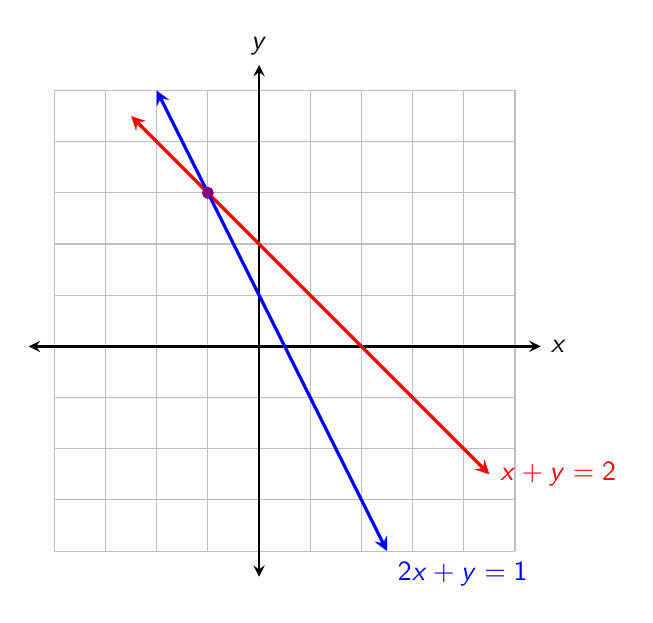
\begin{tikzpicture}[scale=0.65]
\draw[gray!50] (-4,-4) grid (5,5);
\draw[<->, thick] (-4.5,0) -- (5.5,0) node [right] {$x$};
\draw[<->, thick] (0,-4.5) -- (0,5.5) node [above] {$y$};
\draw[<->, very thick, red] (4.5,-2.5) node [right] {$x+y=2$} -- (-2.5,4.5);
\draw[<->, very thick, blue, domain=-2:2.5] plot (\x, -2*\x+1) node [below right] {$2x+y=1$};
\draw[color=violet,fill=violet] (-1,3) circle [radius=3pt];
\end{tikzpicture}
\end{center}

\newpage

Previously, we looked at matrix multiplication. The system of equations
\begin{center}
    \systeme{x+y=2, 2x+y=1}
\end{center}
in matrix form is
\[
\begin{bmatrix}
1 & 1 \\
2 & 1 
\end{bmatrix}
\begin{bmatrix}
x \\ y
\end{bmatrix}
=
\begin{bmatrix}
2 \\ 1
\end{bmatrix}
\qquad \text{or} \qquad
x\begin{bmatrix} 1 \\ 2 \end{bmatrix} + y \begin{bmatrix} 1 \\ 1 \end{bmatrix} = \begin{bmatrix} 2 \\ 1 \end{bmatrix}
\]

\vspace{1.5in}

Transforming $\hat{\imath}$ and $\hat{\jmath}$ by the matrix $\begin{bmatrix} 1 & 1 \\ 2 & 1 \end{bmatrix}$, we get 
\begin{center}
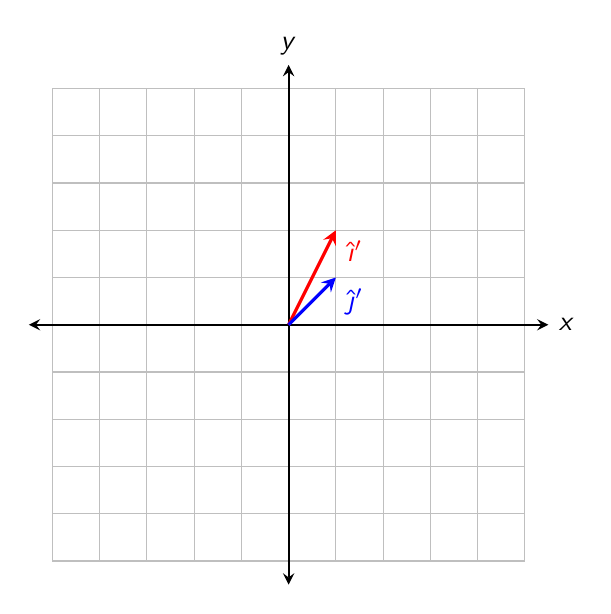
\begin{tikzpicture}[scale=0.6]
\draw[gray!50] (-5,-5) grid (5,5);
\draw[<->, thick] (-5.5,0) -- (5.5,0) node [right] {$x$};
\draw[<->, thick] (0,-5.5) -- (0,5.5) node [above] {$y$};
\draw[->, very thick, red] (0,0) -- (1,2) node [below right] {$\hat{\imath}'$};
\draw[->, very thick, blue] (0,0) -- (1,1) node [below right] {$\hat{\jmath}'$};
\end{tikzpicture}
\end{center}

\vfill

\newpage

\underline{Using these vectors}, we want to get to the point $(2,1)$:
\begin{center}
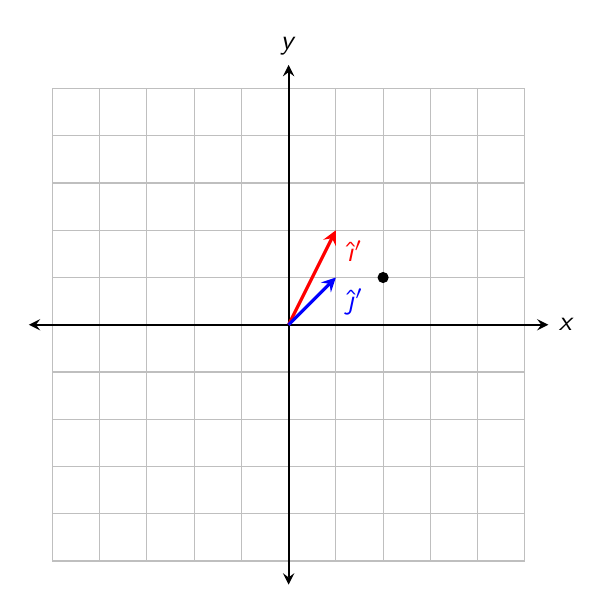
\begin{tikzpicture}[scale=0.6]
\draw[gray!50] (-5,-5) grid (5,5);
\draw[<->, thick] (-5.5,0) -- (5.5,0) node [right] {$x$};
\draw[<->, thick] (0,-5.5) -- (0,5.5) node [above] {$y$};
\draw[->, very thick, red] (0,0) -- (1,2) node [below right] {$\hat{\imath}'$};
\draw[->, very thick, blue] (0,0) -- (1,1) node [below right] {$\hat{\jmath}'$};
\draw[fill=black] (2,1) circle [radius=3pt];
\end{tikzpicture}
\end{center}

\vspace{1.5in}

Knowing our solution is $(-1,3)$:
\[
-1\begin{bmatrix} 1 \\ 2 \end{bmatrix} + 3 \begin{bmatrix} 1 \\ 1 \end{bmatrix} = \begin{bmatrix} 2 \\ 1 \end{bmatrix}
\]

\vfill
Visually, we get
\begin{center}
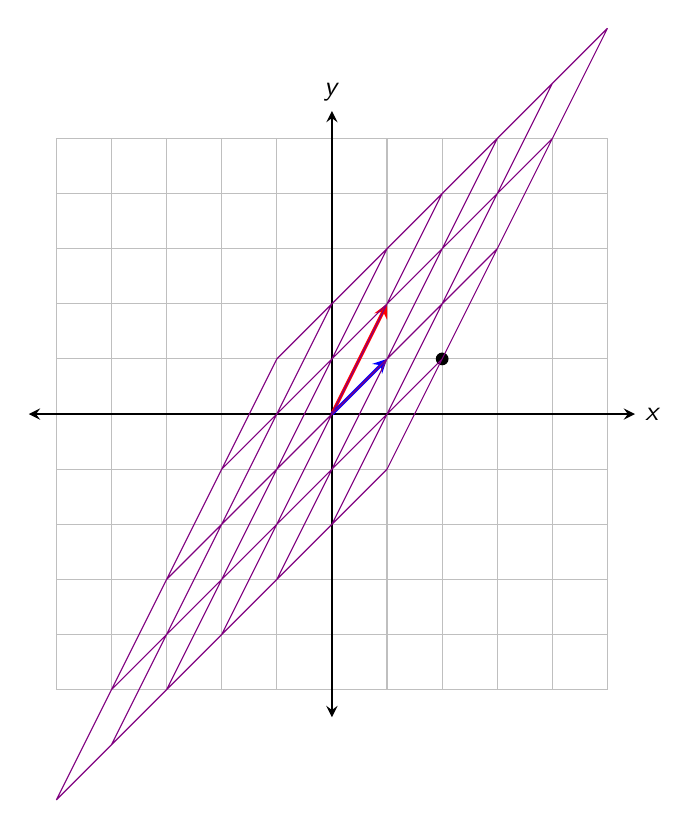
\begin{tikzpicture}[scale=0.7]
\draw[gray!50] (-5,-5) grid (5,5);
\draw[<->, thick] (-5.5,0) -- (5.5,0) node [right] {$x$};
\draw[<->, thick] (0,-5.5) -- (0,5.5) node [above] {$y$};
\draw[->, very thick, red] (0,0) -- (1,2);
\draw[->, very thick, blue] (0,0) -- (1,1);
\draw[fill=black] (2,1) circle [radius=3pt];
% \draw[->, very thick, dashed, red] (0,0) -- (-1,-2) node [above left] {$-1\hat{\imath}'$};
% \draw[->, very thick, dashed, blue] (-1,-2) -- (0,-1);
% \draw[->, very thick, dashed, blue] (0,-1) -- (1,0);
% \draw[->, very thick, dashed, blue] (1,0) -- (2,1) node [below right] {$3\hat{\jmath}'$};
\pgftransformcm{1}{2}{1}{1}{\pgfpoint{0cm}{0cm}}
\draw[violet] (-2,-3) grid (2,3);
\end{tikzpicture}
\end{center}


\newpage

{\color{red}\textbf{Example 1.}} Using the new basis vectors $\hat{\imath} = \begin{bmatrix} 1 \\ 2 \end{bmatrix}$ and $\hat{\jmath} = \begin{bmatrix} 1 \\ 1 \end{bmatrix}$ \newline\\ show that $(2,-1)$ is the solution to  \systeme{x+y=1, 2x+y=3}
\bigskip

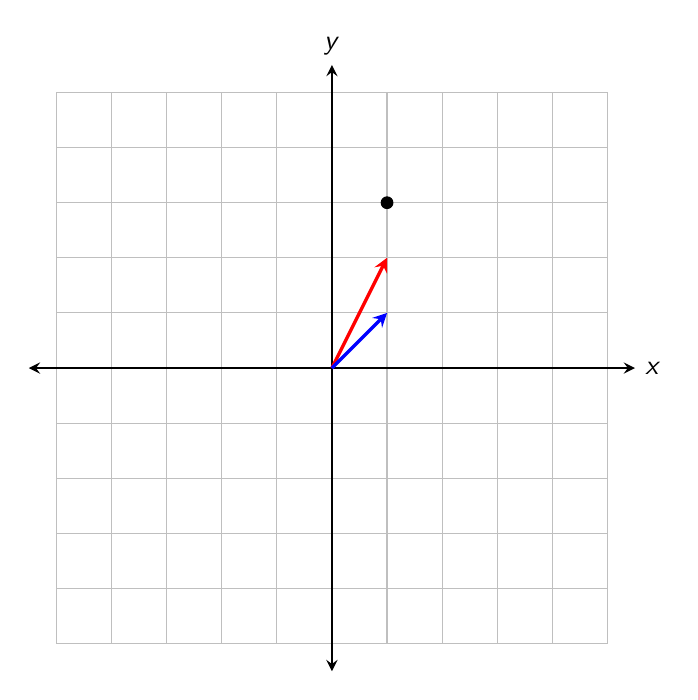
\begin{tikzpicture}[scale=0.7]
\draw[gray!50] (-5,-5) grid (5,5);
\draw[<->, thick] (-5.5,0) -- (5.5,0) node [right] {$x$};
\draw[<->, thick] (0,-5.5) -- (0,5.5) node [above] {$y$};
\draw[->, very thick, red] (0,0) -- (1,2);
\draw[->, very thick, blue] (0,0) -- (1,1);
\draw[fill=black] (1,3) circle [radius=3pt];
\end{tikzpicture}


\vfill

\newpage

Like single equations, some systems of equations have special answers 
\begin{itemize}
    \item No solution: $\varnothing$
    \item Infinite number of solutions
\end{itemize}
\vfill

{\color{red}\textbf{Example 2.}} Using the new basis vectors $\hat{\imath} = \begin{bmatrix} 1 \\ 2 \end{bmatrix}$ and $\hat{\jmath} = \begin{bmatrix} 1 \\ 2 \end{bmatrix}$ show that the system below has no solution.    \newline\\
\systeme{x+y=2, 2x+2y=1}

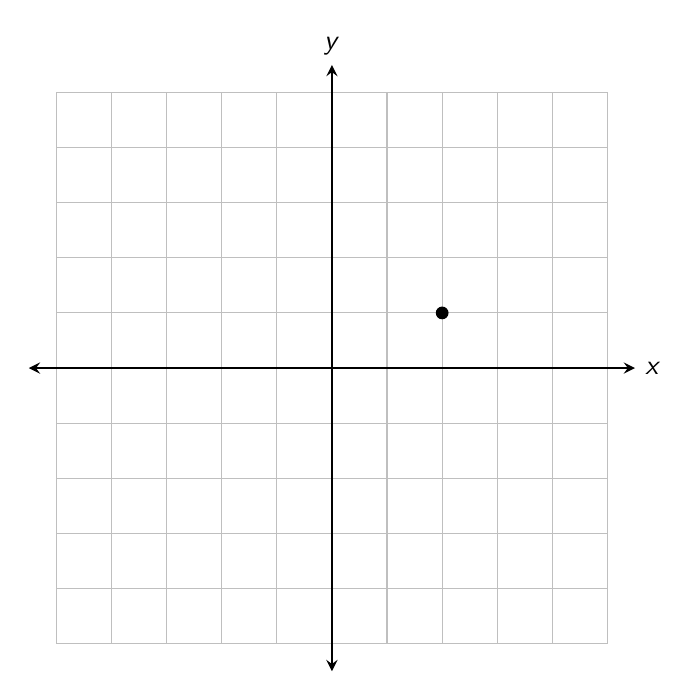
\begin{tikzpicture}[scale=0.7]
\draw[gray!50] (-5,-5) grid (5,5);
\draw[<->, thick] (-5.5,0) -- (5.5,0) node [right] {$x$};
\draw[<->, thick] (0,-5.5) -- (0,5.5) node [above] {$y$};
% \draw[->, very thick, red] (0,0) -- (1,2);
% \draw[->, very thick, blue] (0,0) -- (1,2);
\draw[fill=black] (2,1) circle [radius=3pt];
\end{tikzpicture}
\vfill

\newpage

$\begin{bmatrix}1 & 1 \\ 2 & 2\end{bmatrix} \begin{bmatrix} x \\ y \end{bmatrix} = \begin{bmatrix} 2 \\ 1 \end{bmatrix}$  \newline\\

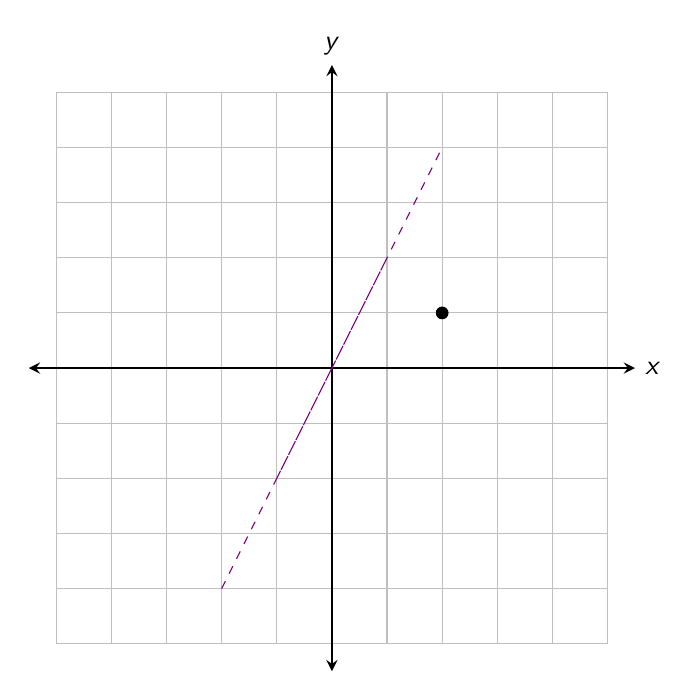
\begin{tikzpicture}[scale=0.7]
\draw[gray!50] (-5,-5) grid (5,5);
\draw[<->, thick] (-5.5,0) -- (5.5,0) node [right] {$x$};
\draw[<->, thick] (0,-5.5) -- (0,5.5) node [above] {$y$};
% \draw[->, very thick, red] (0,0) -- (1,2);
% \draw[->, very thick, blue] (0,0) -- (1,2);
\draw[fill=black] (2,1) circle [radius=3pt];
% \draw[->, very thick, dashed, red] (0,0) -- (-1,-2) node [above left] {$-1\hat{\imath}'$};
% \draw[->, very thick, dashed, blue] (-1,-2) -- (0,-1);
% \draw[->, very thick, dashed, blue] (0,-1) -- (1,0);
% \draw[->, very thick, dashed, blue] (1,0) -- (2,1) node [below right] {$3\hat{\jmath}'$};
\pgftransformcm{1}{2}{1}{2}{\pgfpoint{0cm}{0cm}}
\draw[dashed, violet] (-1,-1) grid (1,1);
\end{tikzpicture}

\vfill

If we graph the equations $x + y = 2$ and $2x + 2y = 1$, we find that the graphs do not intersect:
\begin{center}
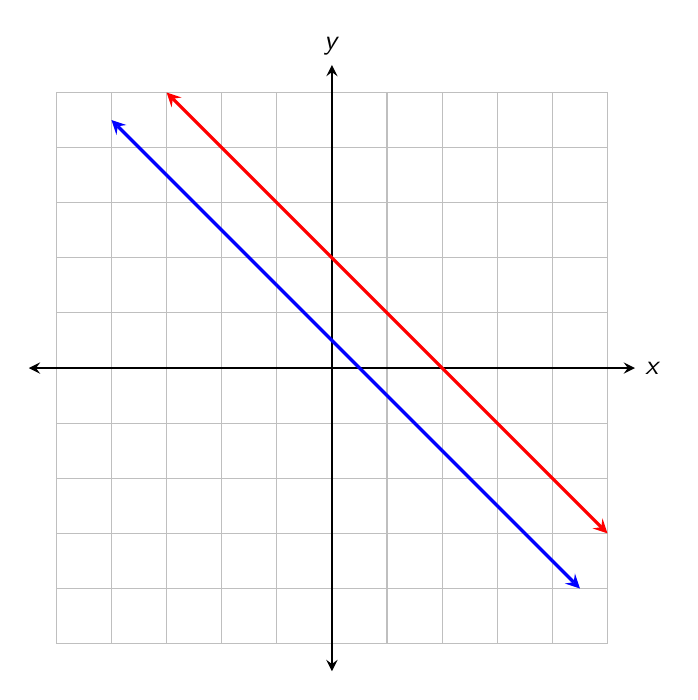
\begin{tikzpicture}[scale=0.7]
\draw[gray!50] (-5,-5) grid (5,5);
\draw[<->, thick] (-5.5,0) -- (5.5,0) node [right] {$x$};
\draw[<->, thick] (0,-5.5) -- (0,5.5) node [above] {$y$};
\draw[<->, red, very thick, domain=-3:5] plot (\x, 2 - \x);
\draw[<->, blue, very thick, domain=-4:4.5] plot (\x, 0.5-\x);
\end{tikzpicture}
\end{center}

\vfill

\newpage

{\color{red}\textbf{Example 3.}} Show that the system below has an infinite number of solutions.    \newline\\

\systeme{2x-y=1, 4x-2y=2}

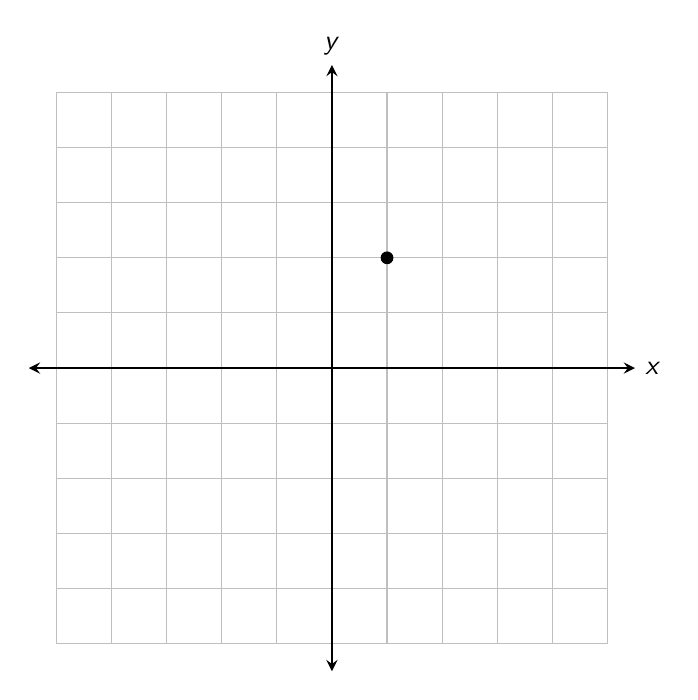
\begin{tikzpicture}[scale=0.7]
\draw[gray!50] (-5,-5) grid (5,5);
\draw[<->, thick] (-5.5,0) -- (5.5,0) node [right] {$x$};
\draw[<->, thick] (0,-5.5) -- (0,5.5) node [above] {$y$};
\draw[fill=black] (1,2) circle [radius=3pt];
\end{tikzpicture}

\vfill

$\begin{bmatrix} 2 & -1 \\ 4 & -2 \end{bmatrix} \begin{bmatrix} x \\ y \end{bmatrix} = \begin{bmatrix} 1 \\ 2 \end{bmatrix}$ \newline\\

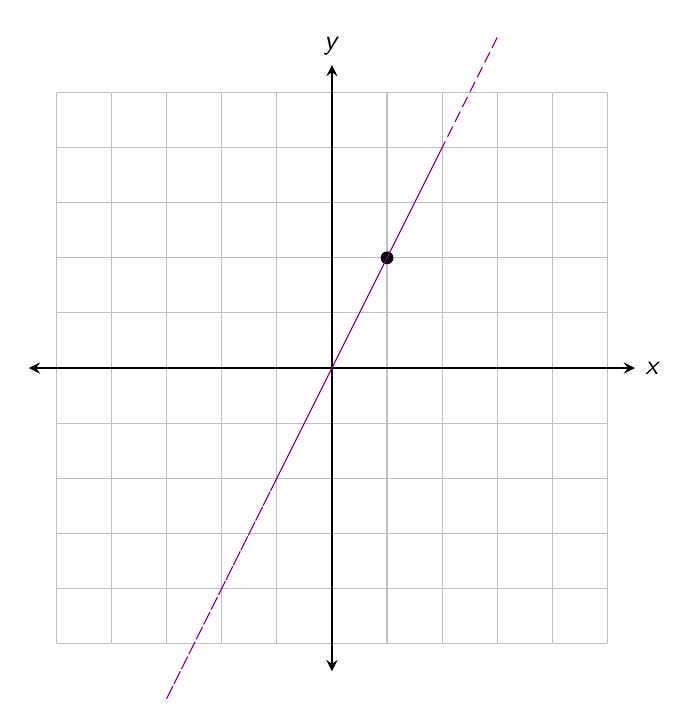
\begin{tikzpicture}[scale=0.7]
\draw[gray!50] (-5,-5) grid (5,5);
\draw[<->, thick] (-5.5,0) -- (5.5,0) node [right] {$x$};
\draw[<->, thick] (0,-5.5) -- (0,5.5) node [above] {$y$};
% \draw[->, very thick, red] (0,0) -- (1,2);
% \draw[->, very thick, blue] (0,0) -- (1,1);
\draw[fill=black] (1,2) circle [radius=3pt];
% \draw[->, very thick, dashed, red] (0,0) -- (-1,-2) node [above left] {$-1\hat{\imath}'$};
% \draw[->, very thick, dashed, blue] (-1,-2) -- (0,-1);
% \draw[->, very thick, dashed, blue] (0,-1) -- (1,0);
% \draw[->, very thick, dashed, blue] (1,0) -- (2,1) node [below right] {$3\hat{\jmath}'$};
\pgftransformcm{2}{4}{-1}{-2}{\pgfpoint{0cm}{0cm}}
\draw[dashed, violet] (-1,-1) grid (1,1);
\end{tikzpicture}

\vfill

\newpage

\subsubsection*{Matrix Methods for Solving a System of Equations}

If we graph the equations $2x-y=1$ and $4x-2y=2$, we find that they are equations for the same line:  \newline\\

\begin{center}
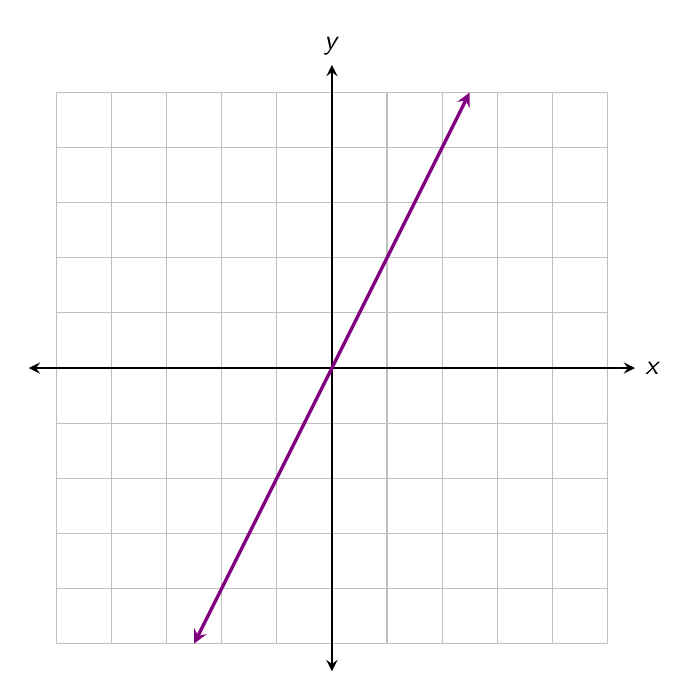
\begin{tikzpicture}[scale=0.7]
\draw[gray!50] (-5,-5) grid (5,5);
\draw[<->, thick] (-5.5,0) -- (5.5,0) node [right] {$x$};
\draw[<->, thick] (0,-5.5) -- (0,5.5) node [above] {$y$};
\draw[<->, very thick, violet, domain=-2.5:2.5] plot (\x, 2*\x);
\end{tikzpicture}
\end{center}

In the intro, we saw that the system of equations   
\begin{center}\systeme{x+y=2, 2x+y=1}\end{center} 
in matrix form is
\[
\begin{bmatrix} 1 & 1 \\ 2 & 1 \end{bmatrix} \begin{bmatrix} x \\ y \end{bmatrix} = \begin{bmatrix} 2 \\ 1 \end{bmatrix}
\]

\vspace{0.75in}

We were able to get a solution $(-1,3)$. 

\vfill 

In matrix form, this is
\begin{flalign*}
\begin{bmatrix}
1 & 0 \\ 0 & 1 
\end{bmatrix}
\begin{bmatrix} x \\ y \end{bmatrix}
=
\begin{bmatrix} -1 \\ 3 \end{bmatrix}   &&\\
\end{flalign*}

\vfill

So, if we can transform 
\begin{flalign*}
\begin{bmatrix} 1 & 1 \\ 2 & 1 \end{bmatrix} \begin{bmatrix} x \\ y \end{bmatrix}
\text{ into }
\begin{bmatrix}
1 & 0 \\ 0 & 1 
\end{bmatrix}
\begin{bmatrix} x \\ y \end{bmatrix}   
&&\\
\end{flalign*}
that will transform the right side (point) we are starting with, $\begin{bmatrix} 2 \\ 1\end{bmatrix}$, to our solution of $\begin{bmatrix} -1 \\ 3 \end{bmatrix}$

\newpage

Another way to look at this is, given $\hat{\imath}'$ and $\hat{\jmath}'$, how can we get back to our original vectors $\hat{\imath}$ and $\hat{\jmath}$ 

\emph{**while using the rules for $\hat{\imath}'$ and $\hat{\jmath}'$**}? \newline\\

\begin{minipage}{0.45\textwidth}
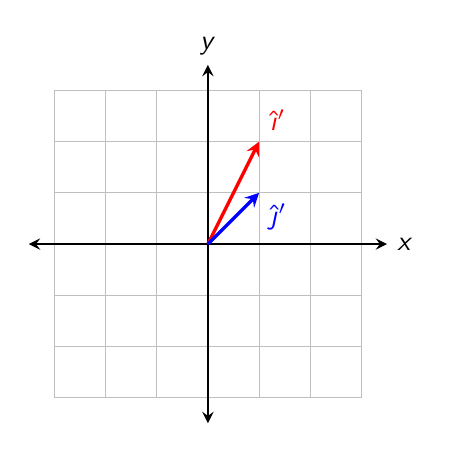
\begin{tikzpicture}[scale=0.65]
\draw[gray!50] (-3,-3) grid (3,3);
\draw[<->, thick] (-3.5,0) -- (3.5,0) node [right] {$x$};
\draw[<->, thick] (0,-3.5) -- (0,3.5) node [above] {$y$};
\draw[->, very thick, red] (0,0) -- (1,2) node [above right] {$\hat{\imath}'$};
\draw[->, very thick, blue] (0,0) -- (1,1) node [below right] {$\hat{\jmath}'$};
\end{tikzpicture}
\end{minipage}
\hspace{-1.25in}
TO $\rightarrow$ \qquad
\begin{minipage}{0.4\textwidth}
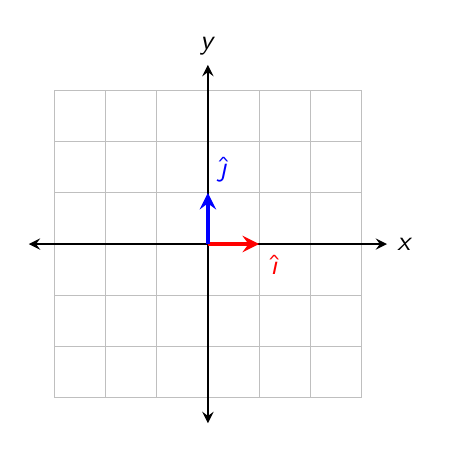
\begin{tikzpicture}[scale=0.65]
\draw[gray!50] (-3,-3) grid (3,3);
\draw[<->, thick] (-3.5,0) -- (3.5,0) node [right] {$x$};
\draw[<->, thick] (0,-3.5) -- (0,3.5) node [above] {$y$};
\draw[->, ultra thick, red] (0,0) -- (1,0) node [below right] {$\hat{\imath}$};
\draw[->, ultra thick, blue] (0,0) -- (0,1) node [above right] {$\hat{\jmath}$};
\end{tikzpicture}
\end{minipage}

\vfill

Multiplying $\hat{\imath}'$ by the vector $\begin{bmatrix} -1 \\ 2 \end{bmatrix}$ gives us the following picture:
\begin{center}
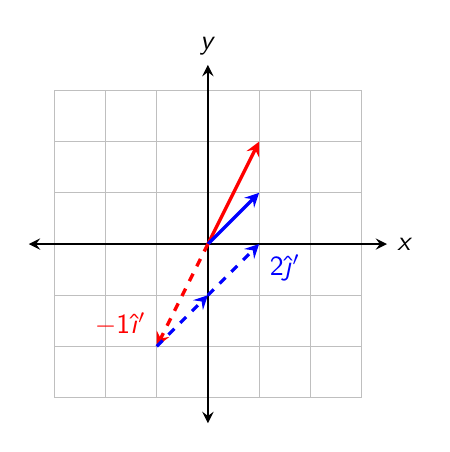
\begin{tikzpicture}[scale=0.65]
\draw[gray!50] (-3,-3) grid (3,3);
\draw[<->, thick] (-3.5,0) -- (3.5,0) node [right] {$x$};
\draw[<->, thick] (0,-3.5) -- (0,3.5) node [above] {$y$};
\draw[->, very thick, red] (0,0) -- (1,2);
\draw[->, very thick, blue] (0,0) -- (1,1);
\draw[->, very thick, red, dashed] (0,0) -- (-1,-2) node [above left] {$-1\hat{\imath}'$};
\draw[->, very thick, blue, dashed] (-1,-2) -- (0,-1);
\draw[->, very thick, blue, dashed] (0,-1) -- (1,0) node [below right] {$2\hat{\jmath}'$};
\end{tikzpicture}
\end{center}

\vfill

Multiplying $\hat{\jmath}'$ by the vector $\begin{bmatrix} 1 \\ -1 \end{bmatrix}$ gives us the following picture:

\begin{center}
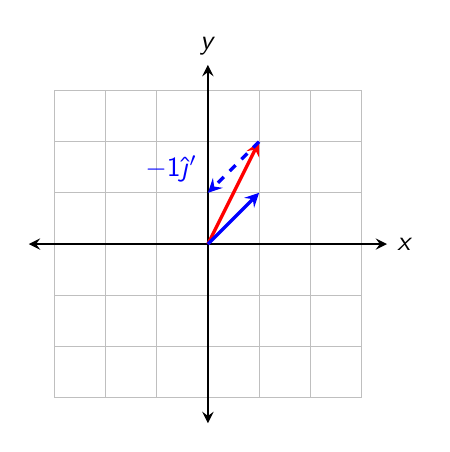
\begin{tikzpicture}[scale=0.65]
\draw[gray!50] (-3,-3) grid (3,3);
\draw[<->, thick] (-3.5,0) -- (3.5,0) node [right] {$x$};
\draw[<->, thick] (0,-3.5) -- (0,3.5) node [above] {$y$};
\draw[->, very thick, red] (0,0) -- (1,2);
\draw[->, very thick, blue] (0,0) -- (1,1);
\draw[->, very thick, blue, dashed] (1,2) -- (0,1) node [above left] {$-1\hat{\jmath}'$};
\end{tikzpicture}
\end{center}

\vfill

\newpage

Putting these ideas together gives us the \textbf{inverse matrix} 
\[
\begin{bmatrix} -1 & 1 \\ 2 & -1 \end{bmatrix}
\]

of $\begin{bmatrix} 1 & 1 \\ 2 & 1 \end{bmatrix}$ which we can then use to solve our system of equations:  \vspace{1in}

\begin{flalign*}
    \begin{bmatrix} -1 & 1 \\ 2 & -1 \end{bmatrix}
    \begin{bmatrix} 1 & 1 \\ 2 & 1 \end{bmatrix}
    \begin{bmatrix} x \\ y \end{bmatrix} &=
    \begin{bmatrix} -1 & 1 \\ 2 & -1 \end{bmatrix}
    \begin{bmatrix} 2 \\ 1 \end{bmatrix} &&\\
    \begin{bmatrix} 1 & 0 \\ 0 & 1 \end{bmatrix}
    \begin{bmatrix} x \\ y \end{bmatrix} &= 
    \begin{bmatrix} -1 \\ 3 \end{bmatrix}   &&\\
    \begin{bmatrix} x \\ y \end{bmatrix} &=
    \begin{bmatrix} -1 \\ 3 \end{bmatrix} &&\\
\end{flalign*}

Which gives us our solution $(-1, 3)$.  \vfill

Working with higher dimension matrices may be more difficult to apply the previous visual techniques. \newline\\

Thus, we can alternatively work with the \emph{rows} of the matrix as well to find our solution. \vfill

To do this, we have 3 \textit{elementary row operations}:
\begin{itemize}
    \item We can interchange 2 rows
    \item We can multiply a row by a nonzero number
    \item We can add (or subtract) two rows
\end{itemize}

\vfill

\newpage

{\color{red}\textbf{Example 4.}} Using elementary row operations, transform the matrix $\begin{bmatrix} 1 & 1 \\ 2 & 1 \end{bmatrix}$ to $\begin{bmatrix} 1 & 0 \\ 0 & 1 \end{bmatrix}$   \vfill

{\color{red}\textbf{Example 5.}} Apply the same elementary row operations from the previous example to the matrix $\begin{bmatrix} 2 \\ 1 \end{bmatrix}$   \vfill

\newpage

{\color{red}\textbf{Example 6.}} Using elementary row operations, transform the matrix $\begin{bmatrix} 1 & 1 \\ 2 & 1 \end{bmatrix}$ to $\begin{bmatrix} 1 & 0 \\ 0 & 1 \end{bmatrix}$  

\vfill

{\color{red}\textbf{Example 7.}} Apply the same elementary row operations from the previous example to the matrix $\begin{bmatrix} 2 \\ 1 \end{bmatrix}$   

\vfill

\newpage

{\color{red}\textbf{Example 8.}} Using elementary row operations, transform the matrix $\begin{bmatrix} 2 & -1 \\ 4 & -2 \end{bmatrix}$ to $\begin{bmatrix} 1 & 0 \\ 0 & 1 \end{bmatrix}$ 
\vfill

{\color{red}\textbf{Example 9.}} Apply the same elementary row operations from the previous example to the matrix $\begin{bmatrix} 1 \\ 2 \end{bmatrix}$   

\vfill


% While graphing methods may be easier for $2 \times 2$ systems of equations, graphing methods get more difficult for larger systems such as $3 \times 3$, $4 \times 4$, etc. We will use elementary row operations and matrices for those.




\end{document}
